\chapter{热膨胀 热传递}

我们知道,物体有冷有热,物体的冷热程度用温度来表示。热的物体温度高,冷的物体温度低。

当物体的温度发生变化时,物体的许多性质也将发生变化。
例如,物体的体积随着温度的升高而增大;
水的温度升高到一定的程度,就要变成水蒸气。
这些跟温度有关的物理现象叫做热现象。

热现象是自然界里很普遍的现象。从这一章开始,我们来学习关于热现象的知识。

\section{物体的热膨胀}\label{sec:2-1}

\begin{wrapfigure}[10]{r}{6cm}
    \centering
    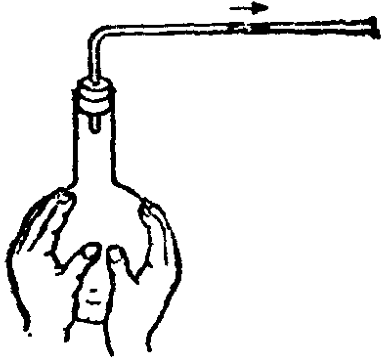
\includegraphics[width=5cm]{../pic/czwl2-ch2-1}
    \caption{气体的热膨胀}\label{fig:2-1}
\end{wrapfigure}

\xiaobiaoti{气体的热膨胀}
把一根弯成直角的玻璃管穿过软木塞插进烧瓶里,
在水平部分的玻璃管里预先装有一段带色的小水柱(图 \ref{fig:2-1})。
被小水柱密封在烧瓶里的空气就是我们要研究的气体。
空气体积的变化,可以从小水柱在玻璃管里的移动看出来。

用手握着烧瓶,使烧瓶里的空气变热,温度升高,就会看到玻璃管里的小水柱向右移动。
这表明空气在温度升高的时候膨胀,体积增大。
手离开后,烧瓶里的空气温度降低,这时小水柱向左移动。
这表明空气在温度降低的时候收缩,体积减小。

在上面的实验里,如果烧瓶里装的不是空气,而是别的任何一种气体,结果也是一样。
因此得到下面的结论:

\CJKunderwave{气体在温度升高的时候膨胀,在温度降低的时候收缩}。


\begin{figure}[htbp]
    \centering
    \begin{minipage}{6cm}
    \centering
    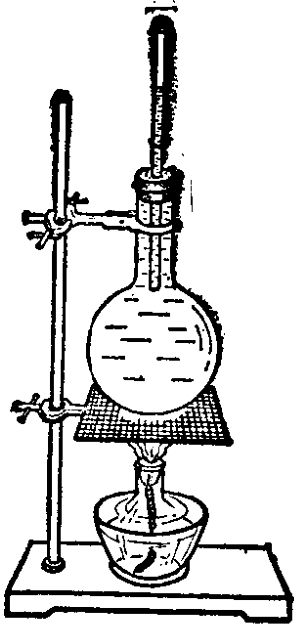
\includegraphics[width=4cm]{../pic/czwl2-ch2-2}
    \caption{液体的热膨胀}\label{fig:2-2}
    \end{minipage}
    \qquad
    \begin{minipage}{8cm}
    \centering
    \vspace{5.5cm}
    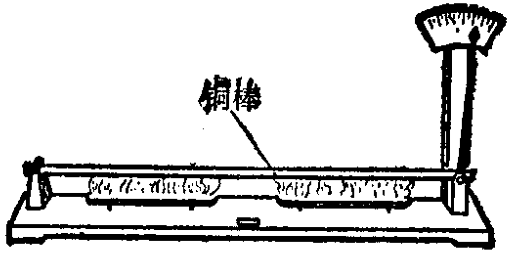
\includegraphics[width=6cm]{../pic/czwl2-ch2-3}
    \caption{固体的热膨胀}\label{fig:2-3}
    \end{minipage}
\end{figure}

\xiaobiaoti{液体的热膨胀}
液体在温度改变的时候,体积也要发生变化。

在烧瓶里装满水或者别的液体,用插有玻璃管的软木塞把瓶口塞紧,液面就升到玻璃管里。
在玻璃管上套上橡皮环,标出这时液面的位置。
对烧瓶加热,使瓶里液体的温度升高,就会看到玻璃管里的液面上升(图 \ref{fig:2-2})。
停止加热,瓶里的液体温度降低,液面又下降。

可见,\CJKunderwave{液体在温度升高的时候膨胀,在温度降低的时候收缩}。

\xiaobiaoti{固体的热膨胀}
如图 \ref{fig:2-3} 所示,铜棒的左端固定,右端放在转轴上,转轴上装着指针。
给铜棒加热,它的温度升高,可以看到指针向右偏,这表明铜棒膨胀了。
停止加热,并在铜棒上盖上浸过冷水的毛巾,使它的温度降低,指针向左偏,这表明铜棒收缩了。
换用其他材料的棒来做这个实验,可以看到同样的现象。

可见,\CJKunderwave{固体在温度升高的时候膨胀,在温度降低的时候收缩}。


在上述实验里,要看出热膨胀现象,
对于气体只要用手加热,气体的温度变化不大;
对于液体要用酒精灯烧,液体的温度变化较大;
对于固体不但要烧,而且要利用指针的偏转把膨胀放大。
这说明气体的热膨胀最显著,液体的热膨胀不如气体显著,固体的热膨胀最不显著。


对于气体、液体和固体的热膨胀,我们得出下面的结论:

\textbf{一般物体都是在温度升高的时候膨胀,在温度降低的时候收缩。
在相同的条件下,固体膨胀得最小,液体膨胀得较大,气体膨胀得最大}。


\section{热膨胀在技术上的意义}\label{sec:2-2}

固体在温度改变的时候,膨胀或者收缩虽然很小,但是如果受到阻碍,产生的力量却很大。
下面,我们做实验来观察固体冷缩时受到阻碍产生的力。

\begin{wrapfigure}[7]{r}{6cm}
    \centering
    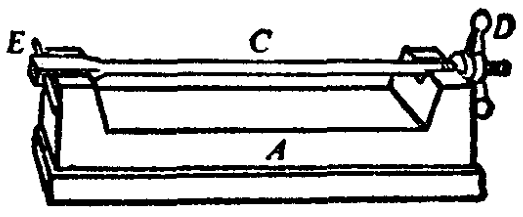
\includegraphics[width=5.5cm]{../pic/czwl2-ch2-4}
    \caption{冷缩时产生的力}\label{fig:2-4}
\end{wrapfigure}

在坚固的生铁座架 $A$上放一根烧得很热的钢棒 $C$ (图 \ref{fig:2-4})。
钢棒的一头有一段生铁棍 $E$,另一头有一个螺旋 $D$ 可以使钢棒卡紧在座架上。
当钢棒冷却收缩时,生铁棍便被拉断。

各种技术设备的温度都要随着气温或工作情况而改变,这就需要我们采取一些办法,
来防止热胀冷缩产生的力的破坏作用。在铺设铁轨的时候,两根铁轨接头的地方要留空隙。
长的铁桥只是一端固定,另一端要架在滚子上(图 \ref{fig:2-5})。这样,当气温变化的时候,
铁轨和铁桥都可以自由伸缩,不致损坏。
工厂里,蒸汽导管的中部装有弯曲的伸缩管(图 \ref{fig:2-6}),当导管里通过高温蒸汽的时候,
导管受热伸长,伸缩管的弯曲程度就改变,使导管不致损坏。

\begin{figure}[htbp]
    \centering
    \begin{minipage}{9cm}
    \centering
    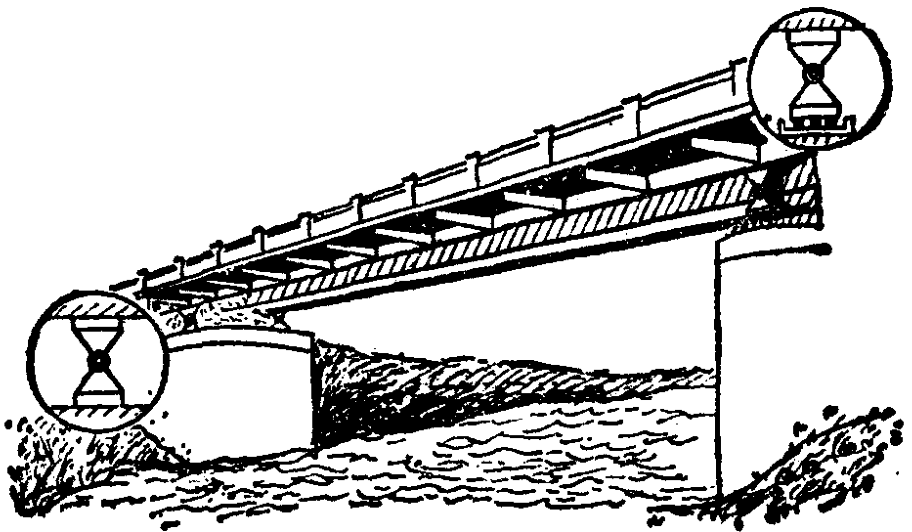
\includegraphics[width=7cm]{../pic/czwl2-ch2-5}
    \caption{铁桥右端架在滚子上}\label{fig:2-5}
    \end{minipage}
    \qquad
    \begin{minipage}{5cm}
    \centering
    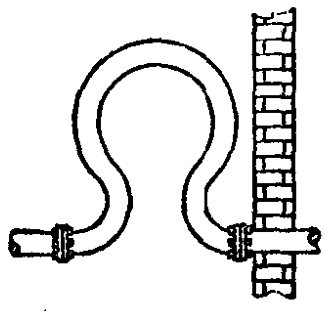
\includegraphics[width=4cm]{../pic/czwl2-ch2-6}
    \caption{伸缩管}\label{fig:2-6}
    \end{minipage}
\end{figure}

技术上也常常利用固体的热膨胀来做有益的事情。
例如,为了使火车车轮耐用,在轮上要套一个硬度大、耐磨损的轮箍。
为了套得紧密,轮箍的内径要做得比车轮稍小一些。
在套轮箍的时候,先把轮箍烧得很热,使它的内径膨胀得比轮子稍大,
然后套在轮子上,轮箍冷却收缩后,就紧紧地箍在车轮上了。
把滚珠轴承装到钢轴上,通常也采用类似的方法,先把轴承浸入热油里,
使它的内径膨胀得比钢轴稍大,然后套在钢轴上。

\begin{wrapfigure}[10]{r}{6cm}
    \centering
    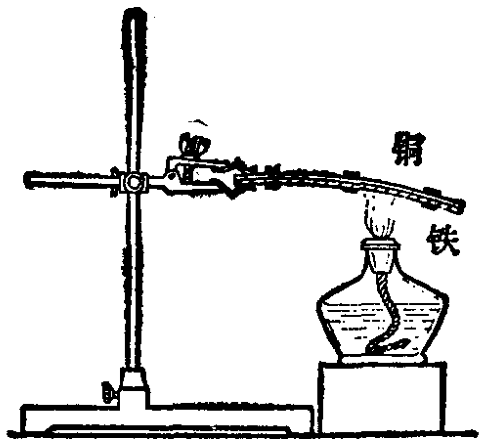
\includegraphics[width=5.5cm]{../pic/czwl2-ch2-7}
    \caption{双金属片}\label{fig:2-7}
\end{wrapfigure}

在相同的条件下,物体的材料不同,热膨胀的大小一般也不相同。
这可以从下面的实验看出来。
把长和宽都相同的铜片和铁片紧紧地铆在一起,做成双金属片。
用酒精灯给双金属片加热,双金属片就向铁片那边弯曲(图 \ref{fig:2-7}),
这表明当同样受热时,铜片膨胀得比铁片大。

各种仪器、机器、建筑物通常都是用不同的材料制成的。
选择这些材料时,必须考虑到它们的热膨胀是不是一样。
例如,在电灯泡上,焊接在玻璃中的那部分金属线,它的热膨胀必须跟玻璃的相等,
这样,温度改变时,金属线和玻璃之间的接合才不会松脱,金属线也不会把玻璃胀破。
在钢筋混凝土建筑物中,钢筋和混疑土的热膨胀也要相同,不然,建筑物就不可能坚固。


\lianxi

(1) 夏天,自行车轮胎里的气如果打得太足,在太阳暴哂下,轮胎容易爆破。为什么?

(2) 乒乓球瘪进去一块,把它浸入开水里烫一下会重新鼓起来。为什么?

(3) 壶里装满冷水,放在火上加热,水会从壶里溢出来。为什么?

(4) 汽油、柴油通常是装在密封的油桶里运输或贮存的。
在向油桶里装油时总要留些空隙,不能装得满满的。为什么?

(5) 为什么混凝土马路每隔一定的距离要留一道缝隙?

(6) 举出两个你知道的利用或防止物体热膨胀的例子。



\section*{小实验}

利用双金属片受热时弯曲的现象,你可以自己做一个自动控制电路。

\begin{figure}[htbp]
    \centering
    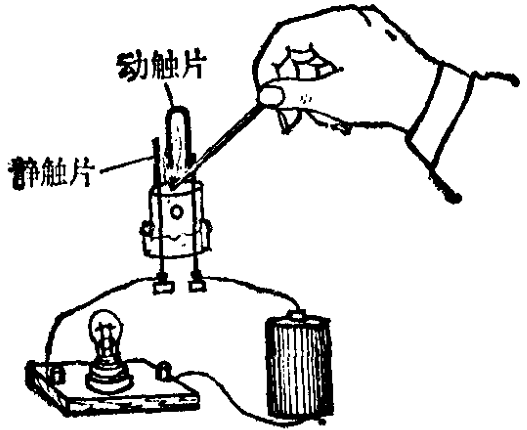
\includegraphics[width=0.5\textwidth]{../pic/czwl2-ch2-8}
    \caption{}\label{fig:2-8}
\end{figure}

找一个废的日光灯起动器,去掉金属(或塑料)外壳,再小心地把玻璃泡打破(注意不要把下边的金属线弄断),
就露出了它的静触片和动触片(图 \ref{fig:2-8})。 U 形的动触片就是双金属片。
照图上画的那样,用导线把起动器、小灯泡和电池连接起来。
点燃火柴去烧动触片,它受热变形跟静触片相接触,于是小灯泡亮了起来。
火柴熄灭后,动触片变冷离开静触片,又恢复到原来的位置,小灯泡就不亮了。

想想看,动触片里面和外面的两种金属,哪一种受热时膨胀得大?

实验中遇到的电路问题,学了电学以后,就会明白了。



\section{温度计}\label{sec:2-3}

\begin{wrapfigure}[30]{r}{6cm}
    \begin{minipage}{2.5cm}
    \centering
    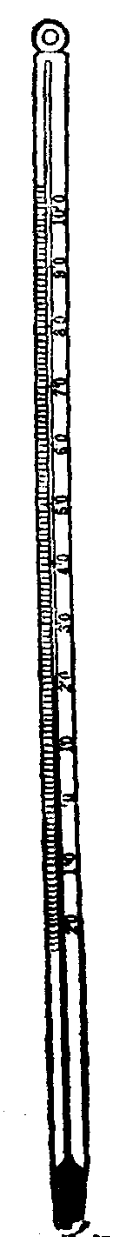
\includegraphics[width=1.5cm]{../pic/czwl2-ch2-9}
    \caption{水银\\温度计}\label{fig:2-9}
    \end{minipage}
    \qquad
    \begin{minipage}{2.5cm}
    \centering
    \vspace{1.8cm}
    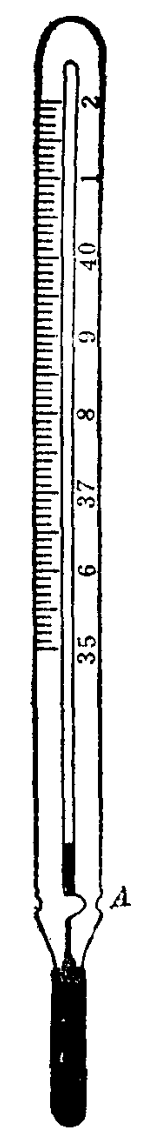
\includegraphics[width=2cm]{../pic/czwl2-ch2-10}
    \caption{体温计}\label{fig:2-10}
    \end{minipage}
\end{wrapfigure}


日常生活中,常用凉、温、烫等词来形容物体的温度。
但是对温度的概念只有这种凭感觉得来的大致的了解,是不够的。
我们要学会准确地测量温度,并且用数值把温度的高低表示出来。
例如,人的正常体温是 37 度,开水的温度是 100 度等。
温度计就是用来测量物体的温度的。

常用的温度计是根据液体热胀冷缩的性质制成的。

实验室里常用的是水银温度计(图 \ref{fig:2-9})。
它的主要部分是一根内径很细而且均匀的玻璃管,管的下端是一个玻璃泡,
在管和泡里有适量的水银,管上标有刻度。
在温度改变时,水银热胀冷缩,管内水银面的位置就随着改变,
从水银达到的刻度就可以读出温度。

常用温度计的刻度,是把冰水混合物的温度规定为 0 度,
把 1 标准气压下的沸水的温度规定为 100 度,
在 0 度和 100 度之间分成 100 等分,每一等分就是 1 度。
这种分度法还可以扩大到 0 度以下和 100 度以上。
用这种办法确定的温度单位叫做\textbf{攝氏度}。
上面提到的人的正常体温和开水的温度,以及日常生活中所说的温度是多少度,都是指摄氏度。

摄氏度用符号 $\celsius$ 来表示。
例如,22 摄氏度就写成 $22\celsius$。
对 $0\celsius$ 以下的温度,还要在度数前边加一个 “$-$” 号。
例如零下 18 摄氏度(或负 18 摄氏度)就写成 $-18\celsius$。

除了水银温度计外,常用的还有酒精温度计、煤油温度计等。
家庭里用来测量气温的温度计,大多是煤油温度计。为了看起来明显,常把煤油染成红色。

温度计不同,测量的范围也不同。
温度计不能用来测量超过它的最高刻度的温度。
因此在使用前应估计被测温度的高低,以免被测温度过高,温度计里的液体把温度计胀破。

温度计能测出物体的温度,是由于温度计的温度能变得与所测物体的温度相同。
因此,使用温度计测量温度时,应使温度计的玻璃泡跟被测物体充分接触。
例如,测量液体的温度时,要使温度计的玻璃泡完全浸没在液体中。
在观察温度计的时候,不要把温度计从液体中拿出来,而应当仍旧放在液体中读数。

医用温度计也叫体温计(图 \ref{fig:2-10}),是用来测量人体温度的。
人体温度的变化一般在 $35\celsius$ 到 $42\celsius$ 之间,
所以体温计的刻度通常是从 $35\celsius$ 到 $42\celsius$。
体温计的泡的容积要比上面的细管的容积大得多,泡里水银的微小膨胀,
就能使细管内水银柱的长度发生显著的变化。
这样就使体温计的测量能准确到十分之一摄氏度。
体温计在 $A$ 点附近管子非常细,水银可以通过这里升到上面去,
温度计离开人体后,水银变冷收缩,水银柱就在这里断开,使上面的水银退不回来。
所以体温计离开人体以后还能表示人体的温度.要使已经升上去的水银再回到泡里,
可以拿着体温计的上部用力往下甩(不是医用的普通温度计不能甩)。

除了上述的液体温度计外,还可以利用物质随温度而改变的其他特性制成其他类型的温度计。



\section{实验:用温度计测量温度}\label{sec:2-4}

温度的测量很重要,但很可能你对温度的估计还是不够准确的。
比如,今天的气温是多少?你每天洗脸用的水的温度是多少?你能说出它们的大约数值吗?
现在我们用温度计来测量一些温度,检查我们估计温度的能力。

先观察一下将要使用的温度计,看看它能够测量的温度范围和每个刻度(每一小格)的温度值,
再回忆一下使用温度计时应该注意的问题。

然后倒一杯开水,用温度计测出它的温度。

让开水冷却到你可以饮用但觉得很烫的程度,估计这时水的温度,再用温度计实际测量。

继续让水冷却,
到你可以饮用而且觉得不烫的程度,
到你的手可以伸进去但觉得很热的程度,
到你的手伸进去觉得不冷不热的程度,
每次都事先估计水的温度,然后用温度计实际测量。

自己设计一个表格,把你每次的估计值和实测数据都填入表中。
比比看,你对温度的估计能力怎样?


\lianxi

(1) 能不能直接用体温计测量开水的温度?为什么?

(2) 利用双金属片可以制成金属温度计(图 \ref{fig:2-11})。
双金属片卷成螺线形,一端固定,另一端用一金属丝绕过转轴拉在弹簧上。
转轴上装有一个指针。从指针的示数可以读出气温。说明这种温度计的原理。
假如跟图中所示的相反,双金属片的内层是铁,外层是铜,温度升高时,指针将向哪边偏转?

\begin{figure}[htbp]
    \centering
    \begin{minipage}{8cm}
    \centering
    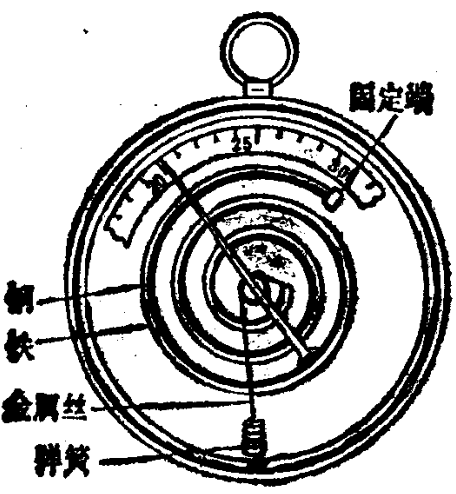
\includegraphics[width=6cm]{../pic/czwl2-ch2-11}
    \caption{}\label{fig:2-11}
    \end{minipage}
    \qquad
    \begin{minipage}{6cm}
    \centering
    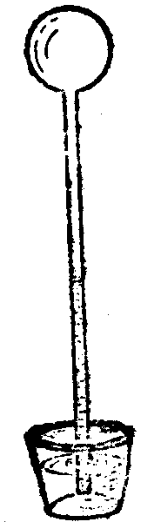
\includegraphics[width=2cm]{../pic/czwl2-ch2-12}
    \caption{}\label{fig:2-12}
    \end{minipage}
\end{figure}

\section*{小实验}

世界上第一个温度计,是伽利略根据气体的热胀冷缩的性质制成的。
它的工作原理如图 \ref{fig:2-12} 所示。
先给球形容器加热,使里面的空气跑出一部分。
停止加热,带色的液体就顺着玻璃管升上去。(为什么?)
这样就做成了一个测量气温的温度计。

想一想,伽利略是根据什么来判断气温高低的?

用这种方法测量气温,要受大气压变化的影响。
想一想,如果气温没有改变而大气压增大或者减小了,观察者将误认为气温发生了什么变化?

你想实验一下伽利略温度计的效果吗?这并不困难。
找一个空的玻璃瓶子,在它的盖子上扎一个小孔。
再找一段透明的管子(例如,拔去头的用完的圆珠笔心),把它的一端插进小孔里。
然后,设法封住瓶盖的缝隙,不让它漏气。
这样,你的伽利略温度计就做成了。


\section{热传递 传导}\label{sec:2-5}

生活经验告诉我们,插在热汤里的金属勺,它的把很快会烫手;
放在炉火上的一壶冷水,不久会被烧开;
坐在篝火旁边的人们,身体会被烤暖。
可见,热可以从温度高的物体传到温度低的物体,或者从物体的高温部分传到低温部分。
这种现象叫做\textbf{热传递}。

实验表明,\CJKunderwave{只要物体之间或同一物体的不同部分存在着温度差,
就会有热传递现象发生,并且将一直继续到温度相同的时候为止}。
由于种种原因,物体之间或同一物体的不同部分,温度常常是不同的。
所以,热传递是一种普遍存在的自然现象。

人们经过长期研究知道,\CJKunderwave{热传递的方式有三种:传导,对流,辐射}。
我们先研究传导。

照图 \ref{fig:2-13} 那样,用凡士林在金属棒上粘几根火柴,然后用酒精灯给金属棒的 $A$ 端加热。
可以看到,离 $A$ 端最近的火柴先掉下,然后其他几根火柴依次掉下,离 $A$ 端越远的火柴掉下得越迟。
这表明,热是从金属棒的温度高的一端沿着金属棒传到温度低的一端去的。

\begin{figure}[htbp]
    \centering
    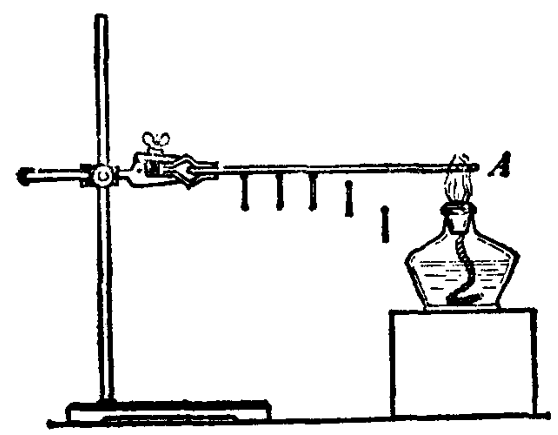
\includegraphics[width=0.5\textwidth]{../pic/czwl2-ch2-13}
    \caption{传导}\label{fig:2-13}
\end{figure}

热从物体的温度较高的部分沿着物体传到温度较低的部分,叫做\textbf{传导}。

各种物质都能够传热,但是不同物质的传热本领不同。

把金属勺放在热汤里面,勺把很快就烫手,可是把瓷勺、木筷子、竹筷子放在热汤里面,
它们很久也不烫手。这表明金属善于传热,瓷、木头和竹子不善于传热。

拿一个装着凉水的试管,照图 \ref{fig:2-14} 那样给试管上部的水加热。
上面的水已经开了,下面的水还不烫手。这表明水不善于传热。

\begin{figure}[htbp]
    \centering
    \begin{minipage}{7cm}
    \centering
    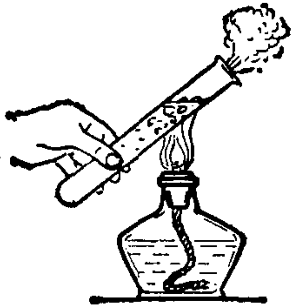
\includegraphics[width=4cm]{../pic/czwl2-ch2-14}
    \caption{水不善于传热}\label{fig:2-14}
    \end{minipage}
    \qquad
    \begin{minipage}{7cm}
    \centering
    \vspace{1cm}
    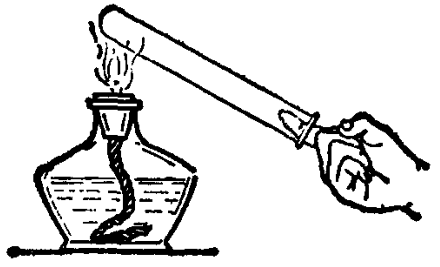
\includegraphics[width=5cm]{../pic/czwl2-ch2-15}
    \caption{空气不善于传热}\label{fig:2-15}
    \end{minipage}
\end{figure}


照图 \ref{fig:2-15} 那样让试管口斜向下方,给试管底部的空气加热,把手指放在试管口处,
过了相当久,手指还不觉得热。这表明空气不善于传热。

我们把善于传热的物质叫做热的良导体。
各种金属都是热的良导体,其中最善于传热的是银,其次是铜和铝。
不善于传热的物质叫做热的不良导体,
瓷、纸、木头、玻璃、皮革都是热的不良导体。
最不善于传热的是羊毛、羽毛、毛皮、棉花、石棉、软木和其他松软的物质。
液体,除了水银以外,都不善于传热,气体比液体更不善于传热。
冬天穿棉衣、皮衣觉得暖和,就是因为在棉花、毛皮的纤维中间有不流动的空气,身体的热不容易散失掉。


\section{对流}\label{sec:2-6}

在图 \ref{fig:2-14} 的实验里,如果我们不是给试管上部的水加热,而是给试管底部的水加热,整个试管中的水都会很快热起来。
同样,在图 \ref{fig:2-15} 的实验里,如果让试管的口向上,给试管底部的空气加热,手指也会很快觉得热了。
既然水和空气都是热的不良导体,那么,在上述情况下,热是怎样传递的呢?

\begin{wrapfigure}[17]{r}{6cm}
    \centering
    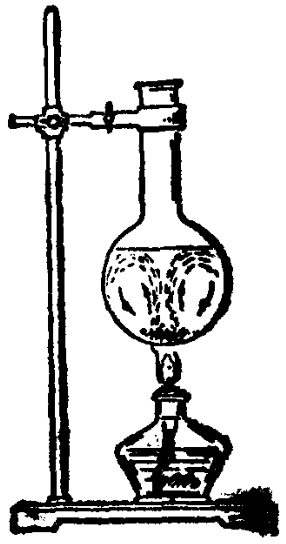
\includegraphics[width=5cm]{../pic/czwl2-ch2-16}
    \caption{水的对流}\label{fig:2-16}
\end{wrapfigure}


如图 \ref{fig:2-16} 所示,把装有冷水的烧瓶悬空架在铁架台上。
水静止后,投入一些高锰酸钾的晶粒,使它沉到瓶底。用酒精灯的小火在烧瓶下面对准晶粒加热。
我们会看到,晶粒周围的紫红色溶液向上升起形成一股股细流,然后又沿瓶的边缘流回瓶底,不一会,
整瓶水都成了紫红色的高锰酸钾溶液。高锰酸钾溶液的流动过程清楚地表示出热传递的情况。
晶粒处的水受热膨胀、密度减小而上升,旁边密度较大的冷水就流过来填补。
流到晶粒处的冷水被加热后又上升,旁边的冷水又流过来填补。这样,水就循环流动起来。
最后,整个烧瓶里的水都变热了。在这里,热是靠水的流动来传递的。

空气的流动也可以传热。例如,冬季用火炉或暖汽片取暖就是靠空气的流动。
火炉或暖汽片使整个屋子空气变暖的过程,同学们可以参照液体流动传热的情况来自己分析。

靠液体或者气体的流动来传递热的方式叫做\textbf{对流}。

根据上面关于对流的讨论知道,要使整个容器中的液体(或气体)的温度很快升高,
应该从下方来加执,因为这样可以形成对流。
我们烧开水的时候,把水壶放在炉火的上面,就是这个道理。

要使整个容器中的液体(或气体)的温度很快降低,应该从上方来冷却,
同样也是因为这样可以形成对流。我们用冰块来冷藏食物的时候,
把冰块放在食物上面比放在下面效果好,就是这个道理。

学过传导和对流以后,我们不难看出它们的区别:
传导是热沿着物体传递的,物质并不流动;
对流是靠物质的流动来传热的。
所以对流是液体、气体特有的传热的方式。



\section*{阅读材料:水的反常膨胀}

在北方,冬季湖水结冰总是从湖面开始,这种现象你不感到奇怪吗?
学过对流以后,爱动脑筋的学生是会感到奇怪的。
因为寒冬降临,冷空气从上方来冷却湖水,假如水总是热胀冷缩,湖水会形成对流,
使全部湖水都降到 $0\celsius$ 而结冰。实际情况为什么不是这样呢?

原来,水的热膨胀有它的特殊性。水在 $4\celsius$ 以上,跟一般的物体一样,是热胀冷缩的,
但是在 $0\celsius$ 到 $4\celsius$ 之间却是热缩冷胀的。
因此,$4\celsius$ 的水无论温升高或降低,体积都要增,密庹都要减小。
就是说,水在 $4\celsius$ 的时候,密度最大。

\begin{figure}[htbp]
    \centering
    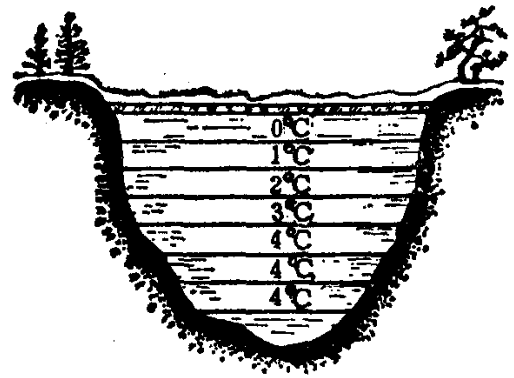
\includegraphics[width=0.3\textwidth]{../pic/czwl2-ch2-17}
    \caption{表面结了冰的湖水的温度}\label{fig:2-17}
\end{figure}

现在我们分析湖水结冰的情况。气温下降时,湖面的水温度也要降低。
在 $4\celsius$ 以上时,由于热胀冷缩,湖面温度较低的水,密度较大要下沉;底部温度较高的水,密度较小,要上升。
这面,湖面较冷的水和底部较暖的水,它们的温度很快就会达到一致了。
湖面的水,当温度降低到 $4\celsius$ 以下时,由于热缩冷胀,密度反而减小,不再下沉,就不再形成对流了。
因此,湖面冷却到结了冰,而底部水的温度仍然可以保持 $4\celsius$ (图 \ref{fig:2-17}),鱼类仍旧可以自由自在地游来游去。



\section*{小实验}

照图 \ref{fig:2-18} 甲那样,在一张厚的图画纸上画线。沿实线剪开,再沿虚线折起,做成一个叶轮。
用细线把叶轮悬起来,在它的下方点燃一根火柴,叶轮就转起来(图乙)。
你自己动手做一做,并说明叶轮为什么会转。

\begin{figure}[htbp]
    \centering
    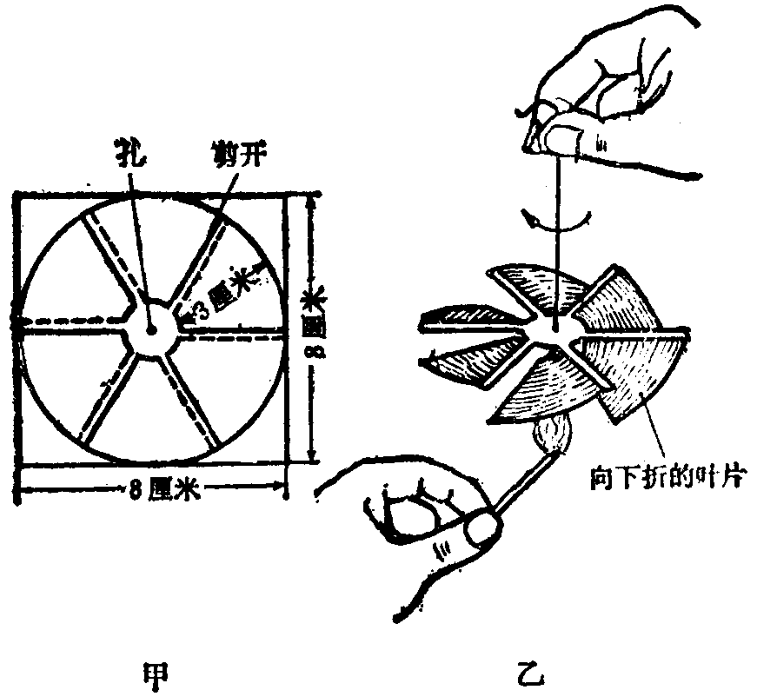
\includegraphics[width=0.5\textwidth]{../pic/czwl2-ch2-18}
    \caption{}\label{fig:2-18}
\end{figure}



\section{辐射}\label{sec:2-7}

放在火炉旁边的物体会被烤热。热是怎样从火炉传到物体的呢?
当然不是由于对流,因为被火炉烤热的空气是上升的。
空气是热的不良导体,传导在这里也不起作用。
如果在火炉和物体之间放一块木板,木板会被烤热,而物体就不会被烤热了。
这表明,热是沿直线从火炉传给物体的。

热由物体沿直线向外射出去,叫做\textbf{辐射}。

跟传导和对流不同,用辐射方式传递热,不需要任何媒介物,可以在真空中进行。
地球上得到的太阳的热,就是通过辐射的方式传来的。

我们的地球每天都吸收太阳辐射来的大量的热。
但是,不同颜色的物体吸收太阳辐射的本领很不相同,下面我们做一个实验来研究这个问题。

\begin{figure}[htbp]
    \centering
    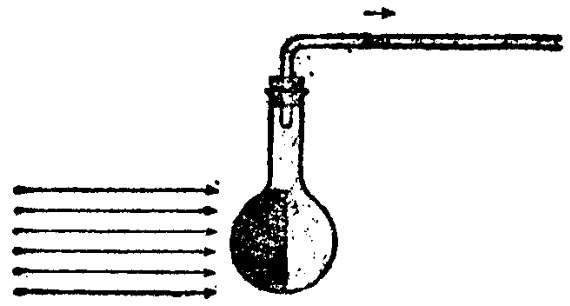
\includegraphics[width=0.5\textwidth]{../pic/czwl2-ch2-19}
    \caption{}\label{fig:2-19}
\end{figure}

利用观察气体热膨胀的实验装置,把烧瓶的一侧涂成黑色,另一侧涂成白色(图 \ref{fig:2-19})。
当太阳光照射黑色一侧时,玻璃管里的小水柱向右移动的距离大。
当太阳光照射白色一侧时,玻璃管里的小水柱向右移动的距离小。
这是因为黑色一侧从太阳辐射中吸收的热多,使烧瓶里空气的温度升得高,体积膨胀得大。
可见,\CJKunderwave{黑色表面的物体对太阳辐射的吸收本领比白色表面的物体强}。
夏天穿浅色衣服比穿深色衣服凉快些,就是这个道理。

物体表面的颜色对吸收太阳辐射有影响这一点,人们常常加以利用。
例如,飞机的表面涂成银白色,可以避免被太阳晒得过热。
相反地,人造地球卫星上的某些部件要利用太阳辐射来加热,就把这些部件涂成黑色。



\section{热传递的利用和防止}\label{sec:2-8}

热传递在日常生活和生产中有广泛的应用。
无论是利用热传递还是防止热传递,传导、对流、辐射这三种方式都应该考虑到,
因为在一般情况下,这三种方式是同时起作用的。

在需要利用热传递来散热的情况下,往往用热的良导体——金属来做热物体的外皮,以加强热的传导。
金属外皮的表面积尽可能做得大些,以增加辐射散热的面积。
此外,还要利用气体或者液体的对流来加快热传递。

汽车发动机工作的时候要发热,使机体的温度不断升高。
但是温度过高,发动机就不能正常工作,这就需要设法散热。
现在我们简单介绍汽车发动机的散热设备(图 \ref{fig:2-20})是怎样利用热传递的。

\begin{figure}[htbp]
    \centering
    \begin{minipage}{8cm}
    \centering
    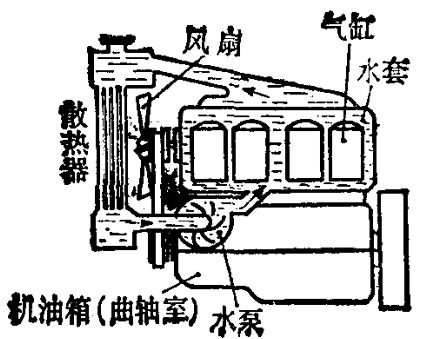
\includegraphics[width=7.5cm]{../pic/czwl2-ch2-20}
    \caption{汽车发动机的散热设备}\label{fig:2-20}
    \end{minipage}
    \qquad
    \begin{minipage}{6cm}
    \centering
    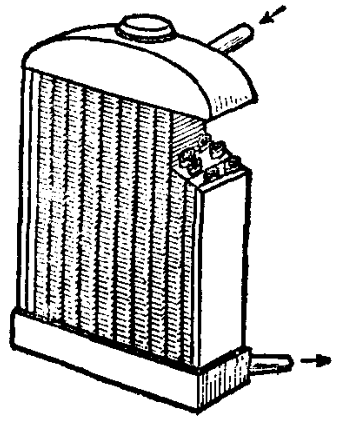
\includegraphics[width=5cm]{../pic/czwl2-ch2-21}
    \caption{散热器}\label{fig:2-21}
    \end{minipage}
\end{figure}


发动机气缸的外面装有水套,水套用上下两根管子跟散热器连通。
水套中的水受热膨胀,从上面的管子流入散热器。
散热器由许多金属管组成(图 \ref{fig:2-21}),金属管的外表面装有很多金属片。
从水套流来的热水经过传导把热传给金属片,金属片再把热向外辐射。
冷却后的水由下面的管子流回水套。
由于水的循环流动,热就不断地被带到散热器散出去。
可以看出,在这种装置里,热传递的三种方式都利用到了。

只利用水的对流来把热带到散热器,散热的速度还是比较慢的。
在功率较大的发动机里,还装有小型水泵,用来加快水的循环流动,使散热加快。
此外,在散热器的附近还装有风扇,把冷空气吹向散热器,这样也可以加快散热的速度。

在需要防止热传递的情况下,就要用相反的方法:
用热的不良导体来包扎物体,尽可能减小物体的表面积,并尽量避免对流的形成。

\begin{wrapfigure}[10]{r}{6cm}
    \centering
    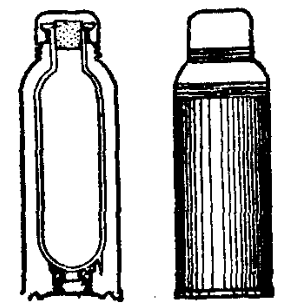
\includegraphics[width=5cm]{../pic/czwl2-ch2-22}
    \caption{保温瓶}\label{fig:2-22}
\end{wrapfigure}


保温瓶(图 \ref{fig:2-22})是防止热传递的例子。
它是一个有双层玻璃壁的瓶子,夹层里的空气已经抽得非常稀薄,接近真空。
夹层内的玻璃壁上镀了银,光亮的象镜子一样。
瓶口盖着软木塞。玻璃和软木都是热的不良导体。
夹层里没有空气,瓶口又盖着塞子,对流不可能发生。
镀银的光亮表面可以把从里面或外面辐射来的热反射回去。
这就是说,保温瓶把热传递的三种方式都尽可能避免了,所以它能够保温。



\lianxi

(1) 在冬天,用手摸户外的东西时,会觉得金属的比木头的凉。为什么?

(2) 盖棉被为什么觉得暖和?在夏天,用棉垫子把冰盖起来,冰是化得快些,还是化得慢些?为什么?

(3) 把滚开的水倒入一个厚玻璃容器时,玻璃容器常常会破裂。为什么?

(4) 图 \ref{fig:2-14} 和图 \ref{fig:2-15} 的实验为什么不发生对流?

(5) 拿一个装满了水的方框形玻璃管 $ABCD$(图 \ref{fig:2-23}),加热它的下角 $A$,玻璃管里的水将怎样流动?

\begin{figure}[htbp]
    \centering
    \begin{minipage}{7cm}
    \centering
    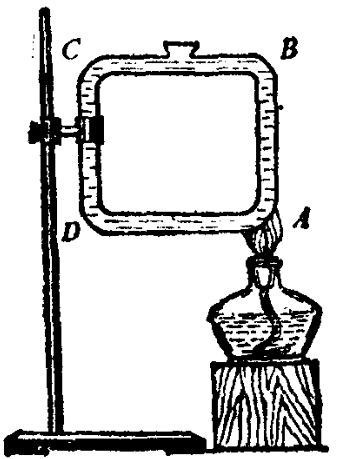
\includegraphics[width=5cm]{../pic/czwl2-ch2-23}
    \caption{}\label{fig:2-23}
    \end{minipage}
    \qquad
    \begin{minipage}{7cm}
    \centering
    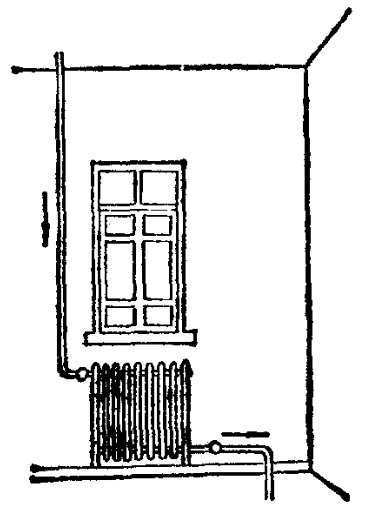
\includegraphics[width=5cm]{../pic/czwl2-ch2-24}
    \caption{}\label{fig:2-24}
    \end{minipage}
\end{figure}

(6) 在图 \ref{fig:2-24} 里,窗子下面是北方房间里冬季供暖用的暖汽片。有人想把它移到窗子上面,使房间宽敞些。
你认为他的想法有什么利弊,说明你的理由。

(7) 在阳光照射下,是脏雪化得快,还是干净雪化得快?

(8) 在夏季,把冰块放在保温瓶里比起放在普通的杯子里,化得快些,还是化得慢些?为什么?

(9) 了解你的教室在冬季(或夏季)采取了哪些取暖(或降温)的措施,并说明这些措施根据的是什么道理。


\section*{复习题}

(1) 举出气体、液体、固体热胀冷缩的实例。气体、液体、固体的热膨胀有什么不同?

(2) 举例说明怎样预防热膨胀所带来的危害?怎样利用热膨胀来做有益的事情?

(3) 采用摄氏度为单位的温度计是怎样确定刻度的?

(4) 使用液体温度计要注意些什么?为什么?

(5) 什么叫做热传递?热传递有哪几种方式?这些热传递的方式各是怎样进行的?

(6) 举例说明怎样尽可能利用或防止热传递?



